%!TEX root = ../Studienarbeit.tex

\chapter{Technische Grundlagen}

\section{Bluetooth}

\subsection{Allgemein}

Bluetooth ist ein Kurzstreckenkommunikationssystem, bei welchen die Hauptmerkmale auf Robustheit, einen geringen Stromverbrauch und geringe Kosten gelegt wurde. Bluetooth wir in zwei Kategorien aufgeteilt. Die erste Kategorie ist \acf{BBR}. Die zweite Kategorie ist \acf{BLE}. Beide Kategorien beinhalten dabei Mechanismen, um Bluetooth-Geräte zu entdecken, einen Verbindungsaufbau durchzuführen sowie eine Verbindung herzustellen. Das Augenmerk bei \ac{BLE} Produkten liegt dabei auf einen niedrigen Stromverbrauch, welche durch eine geringere Datenrate und eine geringere Einschaltdauer während den Datenaustausch als bei \ac{BBR} realisiert wird. Die Übertragungsrate bei \ac{BLE} in der physikalischen Schicht beträgt 2~MB/s. Zu beachten ist, dass ein Bluetooth-Controller entweder nur \ac{BLE}, \ac{BBR} oder beide Bluetooth-Kategorien unterstützen kann. \cite[S.~187]{bluetoothCore}

Die Übertragungsfrequenz von \ac{BLE} ist im lizenzfreien 2.4~GHz ISM-Band von 2402~MHz bis 2480~MHz \cites[S.~4]{siliconBLE}[S.~190]{bluetoothCore}. Das Frequenzband ist in 40 physikalische Kanäle mit jeweils einer Bandbreite von 2~MHz aufgeteilt, wie in Abbildung \ref{fig:frequenzbandBLE} zu sehen ist \cite[S.~190]{bluetoothCore}. Drei dieser 40 physikalischen Kanäle sind für das sogenannte Advertising vorhanden \cite[S.~190]{bluetoothCore}, welches für die Geräteentdeckung, den Verbindungsaufbau und für das Broadcasting von Nachrichten vorhanden ist \cite[S.~4]{siliconBLE}. Die restlichen Kanäle sind für eine allgemeine Datenübertragung vorhanden \cite[S.~190]{bluetoothCore}. Zusätzlich zu der Aufteilung des Frequenzbandes in Kanäle werden Kanäle in Zeiteinheiten aufgeteilt, welche Events genannt werden \cite[S.~190]{bluetoothCore}. Daten werden in Paketen innerhalb eines Events übertragen. Zusätzlich wird bei der Übertragung von Daten Frequenzhopping betrieben, welches zu Beginn jedes Events stattfindet \cite[S.~190f.]{bluetoothCore}. 

\todo[inline]{Bild anpassen und schreiben, abgewandelt von ...}
\begin{figure}[h]
\centering
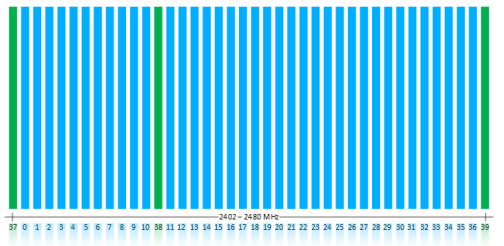
\includegraphics[height=.3\textwidth]{frequenzband}
\caption{Frequenzband mit Kanälen von \ac{BLE} \cite[S.~4]{siliconBLE}}
\label{fig:frequenzbandBLE}
\end{figure}

Die Kompatibilität zwischen Bluetooth-Geräten wird durch sogenannte Profile sichergestellt. Profile beschreiben dafür Funktionen und Eigenschaften von jeder Schicht im Bluetoothsystem \cite[S.~277]{bluetoothCore}. Ebenso werden die benötigten Nachrichten und Prozeduren für die verwendeten Profile durch die Bluetooth \acf{SIG} spezifiziert \cite[S.~1241]{bluetoothCore}.

Bluetooth-Geräten werden unterschiedliche Rollen zugewiesen. Dafür gibt es die Rollen Observer, Broadcaster, Central und Peripheral. Ein Gerät in der Rolle Broadcaster verschickt Advertising-Pakete und ein Gerät welches nur Advertising-Pakete empfangen kann hat die Observer Rolle. So kann eine einseitige Kommunikation zweischen Geräten mittels Advertising-Paketen erfolgen. Eine andere Art der Kommunikation ist mittels einer Verbindung bei dem das Initiatorgerät eine Verbindungsanfrage eines Broadcastergeräts annimt. Daraufhin bekommt das Initiatorgerät die Rolle Central und das Gerät welches ursprünglich in der Rolle Broadcaster war, die Rolle Peripherial. Anzumerken ist, dass ein Gerät zu jeder Zeit mehrere Rollen unterstützen kann, welche jedoch alle der Bluetooth-Controller unterstützen muss. \cite[S.~190f., S.~278, S.~1246ff.]{bluetoothCore}

\subsection{Benötigte Komponenten eines \ac{BLE}-Geräts}

Ein \ac{BLE}-Gerät benötigt einen Mindestumfang an Funktionen damit es laut Bluetooth \ac{SIG} \ac{BLE} kompatibel ist. In Abbildung \todo{Referenz hinzufügen} sind die benötigten Funktionen und deren Zusammespiel durch ein Schichtenmodell dargestellt. Die Funktionen können dabei in einen Hostteil und einen Controllerteil aufgeteilt werden. Im Hostteil befinden sich die Funktionen \acf{L2CAP}, \acf{GAP}, \acf{ATT}, \acf{GATT}, \acf{SDP} und \acf{SMP}. Im Controllerteil befinden sich die Funktionen \acf{PHY} und \acf{LL}. Die Kommunikation zwischen den Hostteil und dem Controllerteil finden mittels dem \acf{HCI} statt \cite[S.~1735]{bluetoothCore}. \cite[S.~193]{bluetoothCore}

\todo[inline]{Bild erstellen}

In den nachfolgenden Unterkapiteln werden die wichtisten Informationen jeder benötigten Funktion von \ac{BLE} beschrieben.

\subsubsection{\acf{PHY}}
Die physikalische Schicht in \ac{BLE} ist zum verschicken und erhalten von Paketen über eines der physikalischen Funkkanäle verantwortlich. \cite[S.~209]{bluetoothCore}

\subsubsection{\acf{LL}}
Die Verbindungsschicht im \ac{BLE}-System besteht aus mehreren Komponenten. Eine Komponente is für die Erstellung, Modefizierung und das Freigeben von logischen Verbindungen zuständig. Eine weitere Komponente ist für das Kodieren und Dekodieren von Bluetooth Paketen zuständig. Auch gibt es eine Komponente welche für die Datenflusskontrolle, die Datenbestätigung und für die Wiederübertragung von Paketen zuständig ist. Die letzte Komponenten in der Verbindungsschicht is für den Zugriff auf das Radiomedium zuständig. Dafür gibt es einen Scheduler, welcher Zeitschlitze des phyiskalischen Mediums an die höherliegenden Dienste veteilt. \cite[S.~207f.]{bluetoothCore}

\subsubsection{\acf{HCI}}
Das \acl{HCI} stellt die Möglichkeit bereit, dass der Hostteil die Funktionen des Controllerteil erreichen kann. Die Übertragung des \ac{HCI} kann dabei wahlweise mittels USB, UART oder anderen Bussystemen stattfinden. \cite[2.~1735f.]{bluetoothCore}